\section{Переход на третий  уровень}

В этой теме переход на третий уровень необычен. Проверочная работа включает в себя не только задачи на тему четности и разбиения на пары, но упражнения на умение видеть аналогии.

Если в группе почти все собираются писать проверочную работу для перехода со 2 уровня на 3, то можно сначала первую часть листка разобрать вместе. Иначе -- отвести больше времени на выполнение работы.

Разберем сначала несколько примеров.

\begin{enumerate}
	\item  Двое играют в следующую игру: первый игрок рисует на клетчатой бумаге квадрат. Затем второй игрок зачеркивает одну из клеток этого квадрата. Потом то же делает первый, и так далее. Проигрывает тот, кто не сможет сделать ход. Кто выиграет при правильной игре и как ему надо играть?
	
	\item  Фрекен Бок и Карлсон играют в фантики. Сначала Карлсон вынимает из кармана несколько фантиков, затем фрекен Бок забирает себе один, затем Карлсон и так далее, пока фантики не кончатся. Проигрывает тот, кто не сможет сделать ход. Кто выиграет при правильной игре и как ему надо играть?
\end{enumerate}

Установление аналогии. Пусть в задаче а) первый не рисует квадрат, а выкладывает фантики в виде квадрата, тогда понятно, что в этом случае «забирание» фантика соответствует зачеркиванию клетки квадрата. Тем самым мы показали, что задачи аналогичны.

\begin{enumerate}
	\item  На прямой отметили несколько точек. После этого между каждыми двумя соседними точками отметили еще по точке. Такое "уплотнение" повторили еще дважды (всего три раза). В результате на прямой оказалось отмечено 4009 точек. Сколько точек было отмечено первоначально?
	
	\item  На квартиры была очередь, и около строящегося дома появился очень странный палаточный городок: все палатки были выстроены в линию. Через некоторое время между каждыми двумя поставили ещё по одной палатке. Через некоторое время -- между каждыми двумя снова по одной. Наконец дом достроили. В нём оказалось 15 этажей, на каждом этаже было 3 квартиры. Каждой семье досталось ровно по одной, и все квартиры оказались заняты. Сколько семей приехало сначала, если в одной палатке жила одна семья?
	
	\item В буфете после городской олимпиады выстроилась очередь за бутербродами. Бутерброды задерживались, и в каждый промежуток между стоящими успело влезть по человеку. Бутерброды все еще не начали выдавать, и во все промежутки опять влезло по человеку, а потом еще по человеку. Тут наконец принесли 4009 бутербродов, и всем стоящим досталось по одному. Сколько человек стояли в очереди первоначально?
\end{enumerate}

Установление аналогии. Заметим, что задачи 1 и 3 полностью аналогичны даже численно. Заменим в задаче 3 людей точками, тогда количество принесенных бутербродов в точности совпадает с окончательным количеством людей в очереди, и мы получим формулировку задачи 1. В задаче 2 общее количество семей закамуфлировано под количество квартир, которое надо сначала вычислить. Сделав это, а также заменив семьи (палатки) точками, мы получим задачу 1 с другими численными данными, в которой «уплотнение» произведено только два, а не три раза.

\begin{enumerate}
	\item  Имеется две кучки 9 камней и 10 камней. За один ход можно взять сколько угодно камней из любой (но только одной) кучки. Проигрывает тот, кто не сможет сделать ход. Кто выигрывает при правильной игре?
	
	\item На шахматной доске размером $ 10\times11 $ в левом нижнем углу стоит ладья. Двое по очереди ходят ею вверх или право (влево и вниз ходить не разрешается). Выигрывает тот, кто первым поставит ладью в правый верхний угол. Кто выигрывает при правильной игре?
\end{enumerate}

Установление аналогии. В этом примере аналогия гораздо менее очевидна, однако она есть. Занумеруем вертикали доски от 0 до 10 (слева направо), а горизонтали от 0 до 9 (снизу вверх). Будем устанавливать соответствие следующим образом: представим себе, что мы играем в обе игры одновременно. Будем двигать ладью вверх, если берут камни из кучки с 9 камнями (назовем эту кучку -- первая) и вправо, если из кучки из 10-ю камнями (назовем эту кучку -- вторая). И, наоборот, при движении ладьи по горизонтали будем брать камни из второй кучки, а при движении по вертикали -- из первой. Каждый раз количество взятых камней равно количеству клеток, на которые переместили ладью. Тем самым мы установили соответствие между позициями двух этих игр.\footnote{ Другими словами: мы задаем координаты ладьи на доске и устанавливаем соответствие позиций следующим образом: позиции ладьи ($  a  $ ; $ b  $) соответствует позиция $  a  $ камней в первой кучке и $  b  $ камней во второй.} 

\head{Сентябрь}{Листок 1.2. Четность. Переводная работа. Аналогии.}
\textit{Как узнать, кто вы -- физик или математик? Предлагается решить простейшую задачу: вскипятить воду, если дано: газовая плита, кран с водой, спички. В этом случае действия физика и математика полностью совпадают. Другая задача: вскипятить воду, если дано: все то же самое, но чайник с водой и газ включен. Что сделает физик? Просто поставит чайник на огонь. Что сделает математик? Выключит газ и выльет воду из чайника, чтобы свести задачу к предыдущей, уже решенной!}	
\begin{flushright}
	Из сборника "Физики шутят."
\end{flushright}
\textbf{Найдите аналогичные между собой и аналогичные задачам из листков 1 и 2 уровня. Обращаем внимание, что числа не обязательно совпадают. Обязательно установите аналогию, как это сделано на примерах. Решать все задачи \underline{не нужно}.}
\begin{enumerate}
	\item На 20 кустах малины, растущих в ряд, количество ягод на любых двух соседних кустах отличается на 1. Можно ли собрать с них 2019 ягод? (Оставлять ягоды на кустах нельзя, они сгниют)
	
	\item У фальшивомонетчиков Гоги и Сереги есть 2018 монет номиналом от 1 до 2018 центов. Они хотят так поделить монеты, чтобы номинальная сумма центов у обоих была одинакова. Удастся ли им это сделать?
	
	\item Воевода и его богатыри питаются золотыми рыбками. Воевода наловил 20 золотых рыбок. Тридцать три богатыря передают друг другу чашу с рыбками, и каждый кладет или забирает из чаши рыбку. Может ли в чаше в результате получиться 10 золотых рыбок?
	
	\item У Лизы в 17 спичечных коробках живут 2010 тараканов. На каждом коробке написано количество проживающих в нем тараканов. Может ли произведение этих чисел быть нечетным числом? Если да, то приведите пример, если нет, то докажите, почему.
	
	\item Может ли окружность пересекать в одной точке (без касания!) все стороны правильного 17-ти угольника?
	
	\item У Ильи есть 2018 стальных шариков весом от 1г до 2018г. Он пытается разложить их на две чашки весов так, чтобы весы оказались в равновесии. Сможет ли он это сделать?
	
	\item Катя вернулась из летнего лагеря и заявила, что в лагере, кроме нее, было еще ровно 2018 ребят, и в начале смены каждый был знаком ровно с тремя. Права ли Катя?
	
	\item Куча семиклассников встали в круг, и каждый из них загадал число. После чего Илья Владимирович прошел круг, и для каждых двух соседей подсчитал произведение их чисел. Если у него получалось отрицательное число, то он ставил обоим этим ребятам по двойке. Всего было поставлено 10 двоек. Докажите, что кто-то из семиклассников загадал ноль. 
	
	\item Злой волшебник пообещал Мефодию Буслаеву власть над миром, если он согнет из волшебной золотой проволоки 2019-тиугольник, длины всех сторон которого составляют нечетное число сантиметров. Волшебник дал ему моток такой проволоки длиной 20 м 8 см и сказал, что проволока обязательно должна быть использована полностью. Сможет ли Мефодий получить власть над миром?
	
	\item Кузнечик прыгает по прямой, причем в первый раз он прыгнул на 1см в какую-то сторону, во второй раз -- на 2см, в третий -- на 3см, и так далее. Докажите, что он не сможет за 2018 прыжков вернуться в начальную точку.
	
	\textbf{Запишите решение задачи  8}
	
\end{enumerate}

Еще раз обращаем внимание, что в данной работе не требуется приводить решения всех задач. Для успешной сдали нужно указать аналогии и записать решение лишь одной задачи.

\section{Решения проверочной работы с уровня 2 на уровень 3}
%
% Тут нужно привести аналогии и решение задачи 1.8
%

Задачи 2 и 6 полностью аналогичны таким образом: монеты -- гири. В обоих задачах требуется разделить их пополам. Также они схожи с задачей 10, в которой прыжок вправо -- монета одному фальшивомонетчику, а прыжок влево - другому. Условие совпадения суммы денег эквивалентно условию попадания в начало координат.
Задача \ref{1.16} аналогична этим трем - 2, 6, 10.

%После урока математики Вася вышел из школы и решил двигаться вдоль проспекта. Сначала он переместился на 1 шаг в какую-то сторону, затем на два шага, потом на 3 и т.д. Сможет ли Вася, сделав в очередной раз 2019 шагов, вернуться в начальную точку?
%
%\begin{prf}	
%	\textbf{1 способ.} Назовем направление вправо положительным, а направление влево - отрицательным. Пусть точка, из которой Вася начал движение, будет начальной. Будем определять в шагах расстояние от начальной точки следующим образом: если Вася идет вправо на какое-то количество шагов n, то будем прибавлять n к уже имеющейся сумме, и вычитать, если он идет влево на n шагов, то вычитать. Таким образом, задача свелась к возможности расставить «плюсы» и «минусы» перед числами от 1 до 2019 так, чтобы в сумме получился ноль. Посмотрим, какие числа вообще могут получаться. Поскольку, среди 2019 последовательных чисел -- 1010 нечетных и 1009 четных, то знакопеременная сумма в любом случае будет нечетной. Следовательно, ноль получить не удастся, так как ноль - число четное.
%	
%	\textbf{2 способ.} Предположим, Васе удалось вернуться в исходную точку. Тогда сумма шагов вправо равна сумме шагов влево. Но тогда сумма всех шагов должна быть четной. Но это не так, поскольку сумма всех натуральных чисел от 1 до 2017 нечетна.
%\end{prf}

\begin{table}[h]\centering
	\begin{tabular}{|c|c|}
		\hline
		номер в проверочной&номер в листках 1.1, 1.2\\
		\hline
		1,3&\ref{an3.2},\ref{1.9},\ref{an1.3}\\
		\hline
		4&\ref{an4.1}\\
		\hline
		5&\ref{an5.1}\\
		\hline
		8&\ref{1.10},\ref{1.11}\\
		\hline
		9&\ref{1.15}\\
		\hline
	\end{tabular}
\end{table}
\begin{prf}
	Задачи 8. Предположим противное, что 0 никто не загадал. Тогда пар соседей, у которых произведение отрицательно четно. Потому что количество пар <<->> <<+>> ровно столько же, сколько пар <<+>> <<->> (если идти, например, по часовой стрелке). А 10 -- это 5 пар. Противоречие.
\end{prf}

\section{Дубль уровня 2}

Второй уровень достаточно сложен. Поэтому скорее всего дубль этого листка потребуется.
\head{Октябрь}{Листок 1. Четность. Уровень 2А}



\begin{thm}
	\label{f1}
	На рисунке прямая пересекает все стороны шестиугольника. Может ли прямая пересекать все стороны какого-нибудь 17-угольника, не проходя ни через одну его вершину?
\end{thm}

%\begin{prf}
%	Заметим, что прямая делит плоскость на две полуплоскости. Отрезок пересекается с такой прямой тогда и только тогда, когда концы отрезка лежат по разные стороны от прямой, то есть в различных полуплоскостях. Поэтому если мы начнем обход многоугольника по часовой стрелке, при переходе к следующей вершине будем менять полуплоскость, в которой находимся. Но тогда первая и семнадцатая вершины окажутся в одной полуплоскости, а значит, отрезок, их соединяющий, не будет пересекаться с прямой. Противоречие.
%\end{prf}

\begin{thm}
	По кругу зацеплены 17 шестерёнок: первая со второй, вторая с третьей, \dots, семнадцатая с первой. Могут ли они вращаться?
\end{thm}

\begin{thm}100 фишек поставлены в ряд. Разрешено менять местами любые две фишки, стоящие через одну. Можно ли поставить фишки в обратном порядке?
\end{thm}

\begin{thm}
	Кузнечик прыгает по прямой, причем в первый раз он прыгнул на 1см в какую-то сторону, во второй раз - на 3см, в третий - на 5см, и так далее. Сможет ли он за 2011 прыжков вернуться в начальную точку?
\end{thm}

\begin{thm}
	В 7Ю учится 30 человек. На каждый день нужно назначить трое дежурных. Можно ли так составить график дежурства, чтобы через некоторое время каждый подежурил с каждым ровно один раз?
\end{thm}

\begin{thm}
	На шахматной доске стоят 17 шашек, расположенных симметрично относительно большой диагонали. Докажите, что есть шашка или шашки и на большой диагонали.
\end{thm}	

\begin{thm}
	Витя и Коля купили несколько шоколадок «Вдохновение»\footnote{Шоколадка «Вдохновение» состоит из нескольких отдельных плиток, каждая из которых содержит две дольки.} и решили их поделить между собой. Каждую плитку брал себе целиком либо Витя, либо Коля, либо они ломали ее пополам. После этого Витя заявил, что Коля взял себе на одну дольку больше. Могло ли такое быть? 
\end{thm}
\begin{figure}[h]\centering
	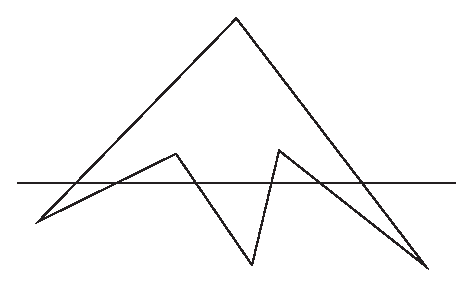
\includegraphics[width=8 cm]{./img/six}
	\caption{\textbf{Задача \ref{f1}}}
\end{figure}

\head{Октябрь}{Листок 1. Четность. Переводная работа 2А. Аналогии.}

\textbf{Найдите аналогичные между собой и аналогичные задачам из листков 1 и 2 уровня. Обращаем внимание, что числа не обязательно совпадают. Обязательно установите аналогию, как это сделано на примерах.}

\textbf{Задача 1A.} У двоечника Вани есть 2019 дневников. Он хочет разложить их по кругу так, чтобы количество двоек в лежащих рядом дневниках отличалось на 1. Сможет ли он это сделать?

\textbf{Задача 2A.} На далекой планете Занзибар живут многоножки. Как-то собрались вместе 2018 многоножек с количеством ножек от 1 до 2018. Причем известно, что у всех количество ножек разное. Они хотят разбиться на две команды для игры в крокет, чтобы общее количество ножек в командах было одинаково. Удастся ли им это сделать?

\textbf{Задача 3A.} Михаил Владимирович написал на доске программу, содержащую 2019 строчек. После чего каждый из 20 учеников 7Ю класса вышел к доске (один или несколько раз) и дописал или стер одну строчку программы. В результате на доске оказалась записанной программа из 17 строчек. Докажите, что нечетное число раз к доске выходило четное число учеников.

\textbf{Задача 4A.} У Жени в 20 аквариумах живут 2019 креветок. На каждом аквариуме написано количество проживающих в нем креветок. Может ли произведение этих чисел быть нечетным числом? Если да, то приведите пример, если нет, то докажите, почему.

\textbf{Задача 5A.} Шахматный конь обошел все клетки шахматной доски 7х7. Мог ли он начать не с угловой клетки, а с соседней с угловой?

\textbf{Задача 6A.} У Ильи есть 2018 стальных шариков весом от 1г до 2018г. Он пытается разложить их на две чашки весов так, чтобы весы оказались в равновесии. Сможет ли он это сделать?

\textbf{Задача 7A.} Незнайка, вернувшись из путешествия, рассказывал, что в некоторой планетарной системе 2019 планет, причем каждая имеет межпланетное сообщение еще с тремя другими. Не заблуждается ли Незнайка?

\textbf{Задача 8A.} Лизочка играет в Зазеркалье. Каждый день она меняем имя. Если она сегодня звалась Лиза, то на следующий день -- Лизавета. Если же сегодня она звалась Лизавета, то на следующий день она зовется Лизой. А еще она меняет цвет платья -- два дня носит красное, а потом два дня -- синее. 1 сентября она назвалась Лизой и пришла в белом, а на следующий день уже надела красное. В каком платье и с каким именем она встретит Новый Год?\footnote{31 декабря} 

\textbf{Задача 9A.} Злой волшебник пообещал Мефодию Буслаеву власть над миром, если он соберет волшебные бусы из 49 камней, чередуя алмаз и бриллиант. Причем, чтобы алмазов было меньше, чем бриллиантов, а начинались бусы с алмаза. Сможет ли Мефодий получить власть над миром?

\textbf{Задача 10A.} Кузнечик прыгает по прямой, причем в первый раз он прыгнул на 1см в какую-то сторону, во второй раз -- на 2 см, в третий -- на 3 см, и так далее. Докажите, что он не сможет за 2010 прыжков вернуться в начальную точку.

\textbf{Задача 11A.} Докажите, что число способов расставить на шахматной доске $ 2018\times2018 $ 2018 ферзей так, чтобы они не били друг друга, четно.

\textbf{Запишите решения задач  8  и  3}
\hrule
